\section{Инфраструктура проекта}

\subsection{Архитекрутра}
За основу берётся архитектурный паттерн \acrshort{mvc}. Он предполагает разделение данных приложения, пользовательского интерфейса и управляющей логики на три отдельных компонента: Модель, Представление и Контроллер – таким образом, что модификация каждого компонента может осуществляться независимо.

\begin{figure}[h]
    \begin{center}
        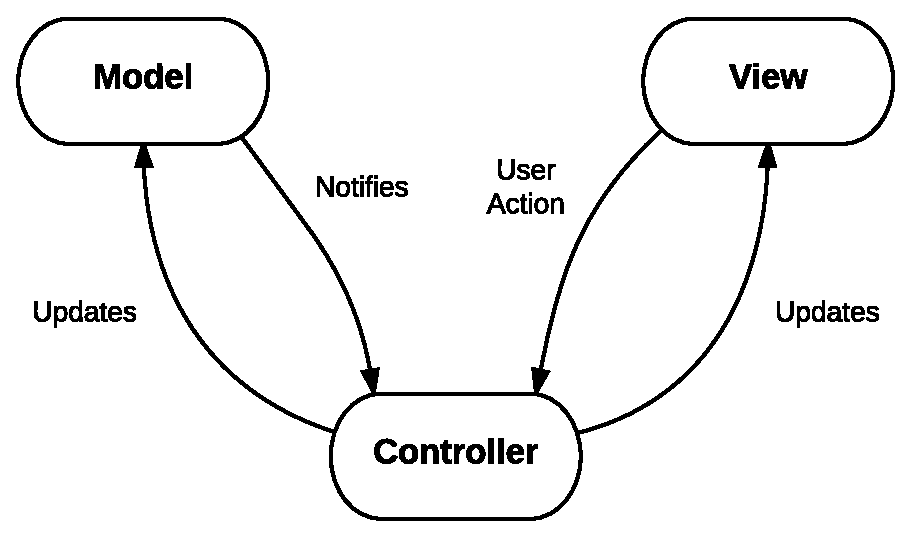
\includegraphics[scale=0.7]{images/MVC-basic.eps}
    \end{center}
    \caption{Визуализация архитектуры \acrshort{mvc}}
\end{figure}

\subsubsection{Связь логических компонетов и применяемых технологих}
\begin{itemize}
    \item Model --- \textcite{seqorm} для сервера и \textcite{redux} для клиента.
    \item View --- \textcite{react}
    \item Controller --- \textcite{express}
\end{itemize}

\subsection{Сущности}
Всегда перед проектированием проекта описывают сущности и их атрибуты. На основе данной информации будет стоится база данных. В моём случае они следующие:

\begin{table}[h!]
    \begin{center}
        \begin{tabular}{|l|p{6.5cm}|}
            \hline
            \multicolumn{1}{|c|}{\textbf{Сущность}} & \multicolumn{1}{c|}{\textbf{Атрибуты}} \\ \hline
            Пользователь & \begin{itemize}
                \item ID пользователя
                \item Логин
                \item Пароль
                \item Email
            \end{itemize} \\ \hline
            Тест & \begin{itemize}
                \item ID теста
                \item Название
                \item Теги
                \item Контент
                \item Ответы
                \item Дата создания
                \item Дата последнего изменения
            \end{itemize} \\ \hline
            Тег & \begin{itemize}
                \item ID тега
                \item Название
            \end{itemize}
            \\ \hline
            Попытка & \begin{itemize}
                \item ID попытки
                \item ID пользователя
                \item ID теста
                \item Результат
                \item Ответы пользователя
                \item Дата прохождения
                \item Время прохождения
            \end{itemize}
            \\ \hline
        \end{tabular}
    \end{center}
    \caption{Описание сущностей и атрибутов}
\end{table}

\subsection{Сборка и запуск}
Все процессы отвечающие за сборку и запуск приложения я разделил на подзадачи. Каждая такая подзадача является npm скриптом. Они все описываются в файле package.json. Также среди данных скриптов можно выделить две группы -- Development и Production.

\subsubsection{Development}
Скрипты из данной группы отвечают за то, чтобы приложение можно было запускать в режиме разработки, а именно:
\begin{enumerate}
    \item сборка клинтской части не занимало слишком много времени
    \item клинет пересобирался при изменении какого-либо файла
    \item сервер перезапускался при изменения кода серверверной части
    \item в браузере были доступны source map
\end{enumerate}

\subsubsection{Production}
Скрипты из данной группы отвечают за то, чтобы приложение можно было запускать в режиме c максимальными оптимизациями, а именно:
\begin{enumerate}
    \item минификация статический файлов
    \item оптимизация работы библиотек
    \item сборка серверной части
\end{enumerate}

\subsection{Деплоинг}


\subsection{Организация работы с \textcite{git}}
\subsubsection{Git Workflow}
Для организации работы с системой контроля версий в проекте используется подход Git Workflow. Он нужен для согласованного и продуктивного выполнения работы.

\begin{figure}[h!]
    \begin{center}
        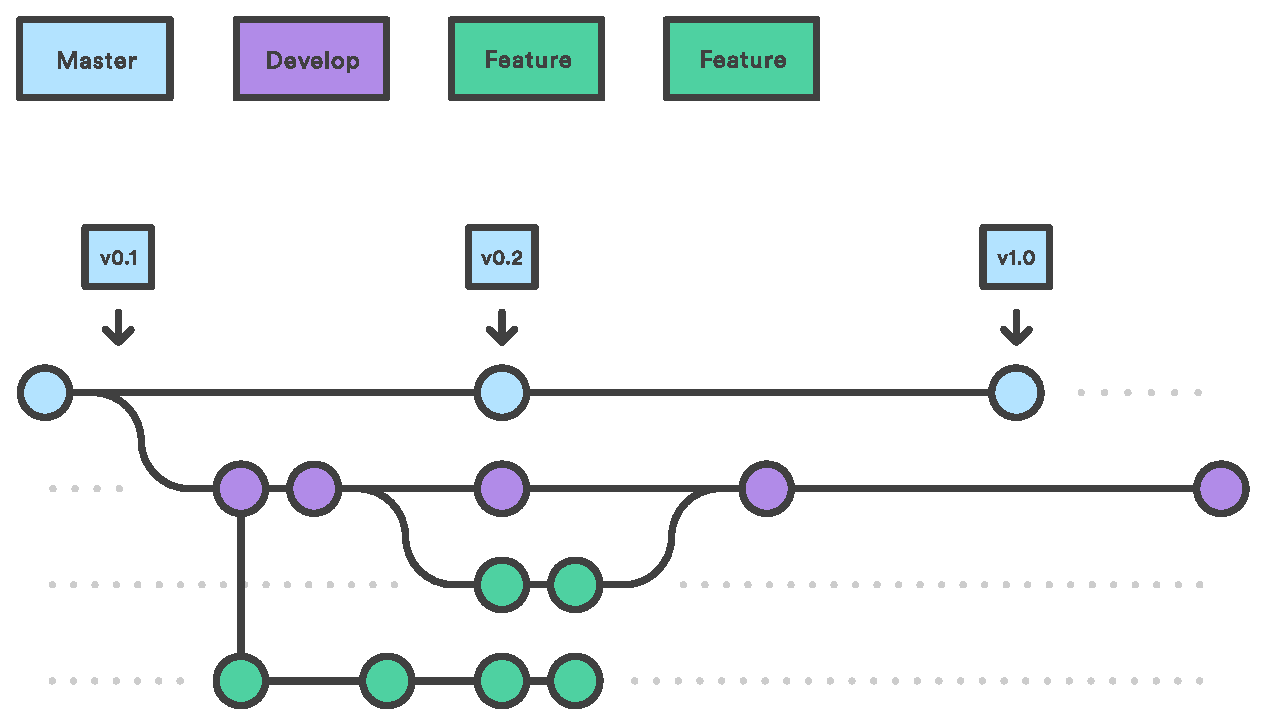
\includegraphics[scale=0.6]{images/git-workflow.eps}
    \end{center}
    \caption{Пример использования подхода Git Workflow}
\end{figure}

\subsubsection{Git hooks}
Чтобы в репозитории хранился код, который проходит проверки линтеров и тестовых фреймворков, нужно использовать Git Hooks. Они позволяют обработать события pre-commit, pre-push, post-commit и так далее.

Есть удобный пакет в npm -- husky. Он позволяет определить в package.json обработку событий. В моём проекте нужно, чтобы на событие pre-commit выполняли проверки линтеры, а потом при успешном результате исполнялись unit-тесты.

\begin{listing}[h!]
\begin{pycode}
import json
from pprint import pprint

with open(f"{PROJECT_PATH}/package.json", "r") as f:
    config = json.load(f)

    print(r"\begin{noerr}")
    print(r"\begin{minted}{json}")
    pprint(config["husky"])
    print(r"\end{minted}")
    print(r"\end{noerr}")
\end{pycode}
\caption{Настройки для Git Hooks}
\end{listing}

\clearpage